\documentclass[]{article}
\usepackage[spanish]{babel}
\usepackage{graphicx}
\usepackage[utf8]{inputenc}
\usepackage{fancyhdr}
\usepackage{lastpage}

\pagestyle{fancy}
\fancyhf{}
\rfoot{Page \thepage\hspace{1pt} de~\pageref{LastPage}}

\title{Practica 7}
\author{Guillermo Lopez Garcia}
\begin{document}
\maketitle

\textbf{Ejercicio 1.} \\

Como se puede apreciar en la gráfica siguiente, el servidor sin pool de hebras cuando la carga aumenta demasiado,
se puede producir bloqueos por el acceso a los recursos compartidos (socket) y crear una tiempo de respuesta
demasiado elevado. Por otra parte, si vemos la solución con pool de hebras, vemos como los tiempos de respuesta
se mantiene, con ligeras variaciones, pero se mantienen casi constantes.

\begin{figure}
  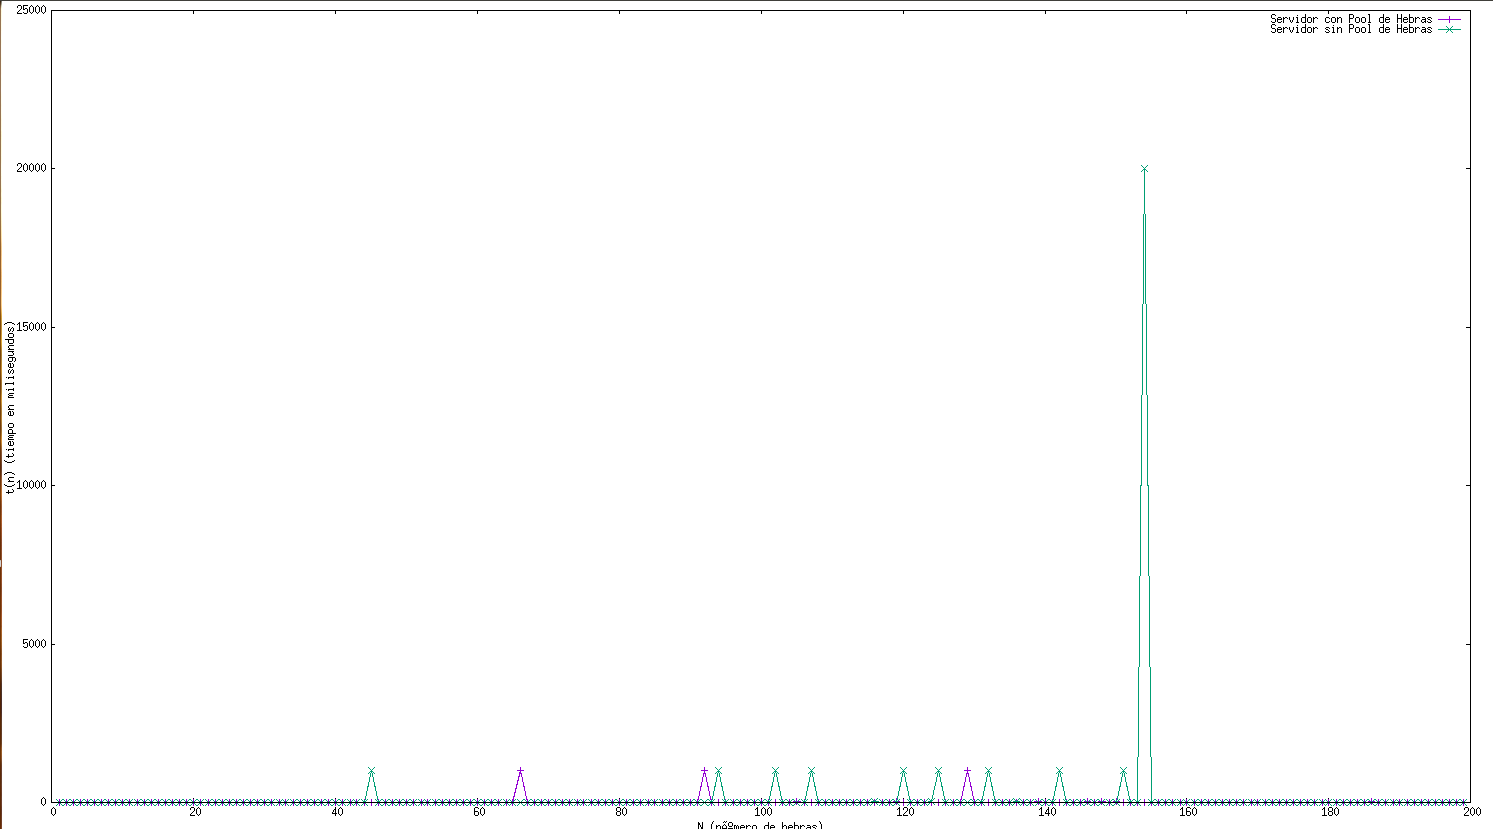
\includegraphics[width=\linewidth]{img.png}
  \caption{Comparativa servidor sin y con pool de hebras}
\label{fig:comp}
\end{figure}
\end{document}
